\chapter{Experiments and results}

\label{ch:Experiments and results}

\setlength{\parindent}{4em}
\setlength{\parskip}{1em}
\renewcommand{\baselinestretch}{1.5}

\section{Hardware for the experiment}

In our project, first we plan how to investigate the EEG data from the subject. There are 2 categories to investigate the data those are software and hardware. When we know like that we go to study how is it different between software and hardware that use in this project and when we already study in it we know that hardware is better than software and we choose it and We plan to design the hardware to use it in experiment.This is materials that we use in our project.

\subsection{EPOC headset by Emotiv}

\subsection{Arduino Uno}

\subsection{Gravitech Gerora WS2812S LED}

\subsection{Visual stimulus (ERP)}
\begin{figure}[ht]
	\centering
	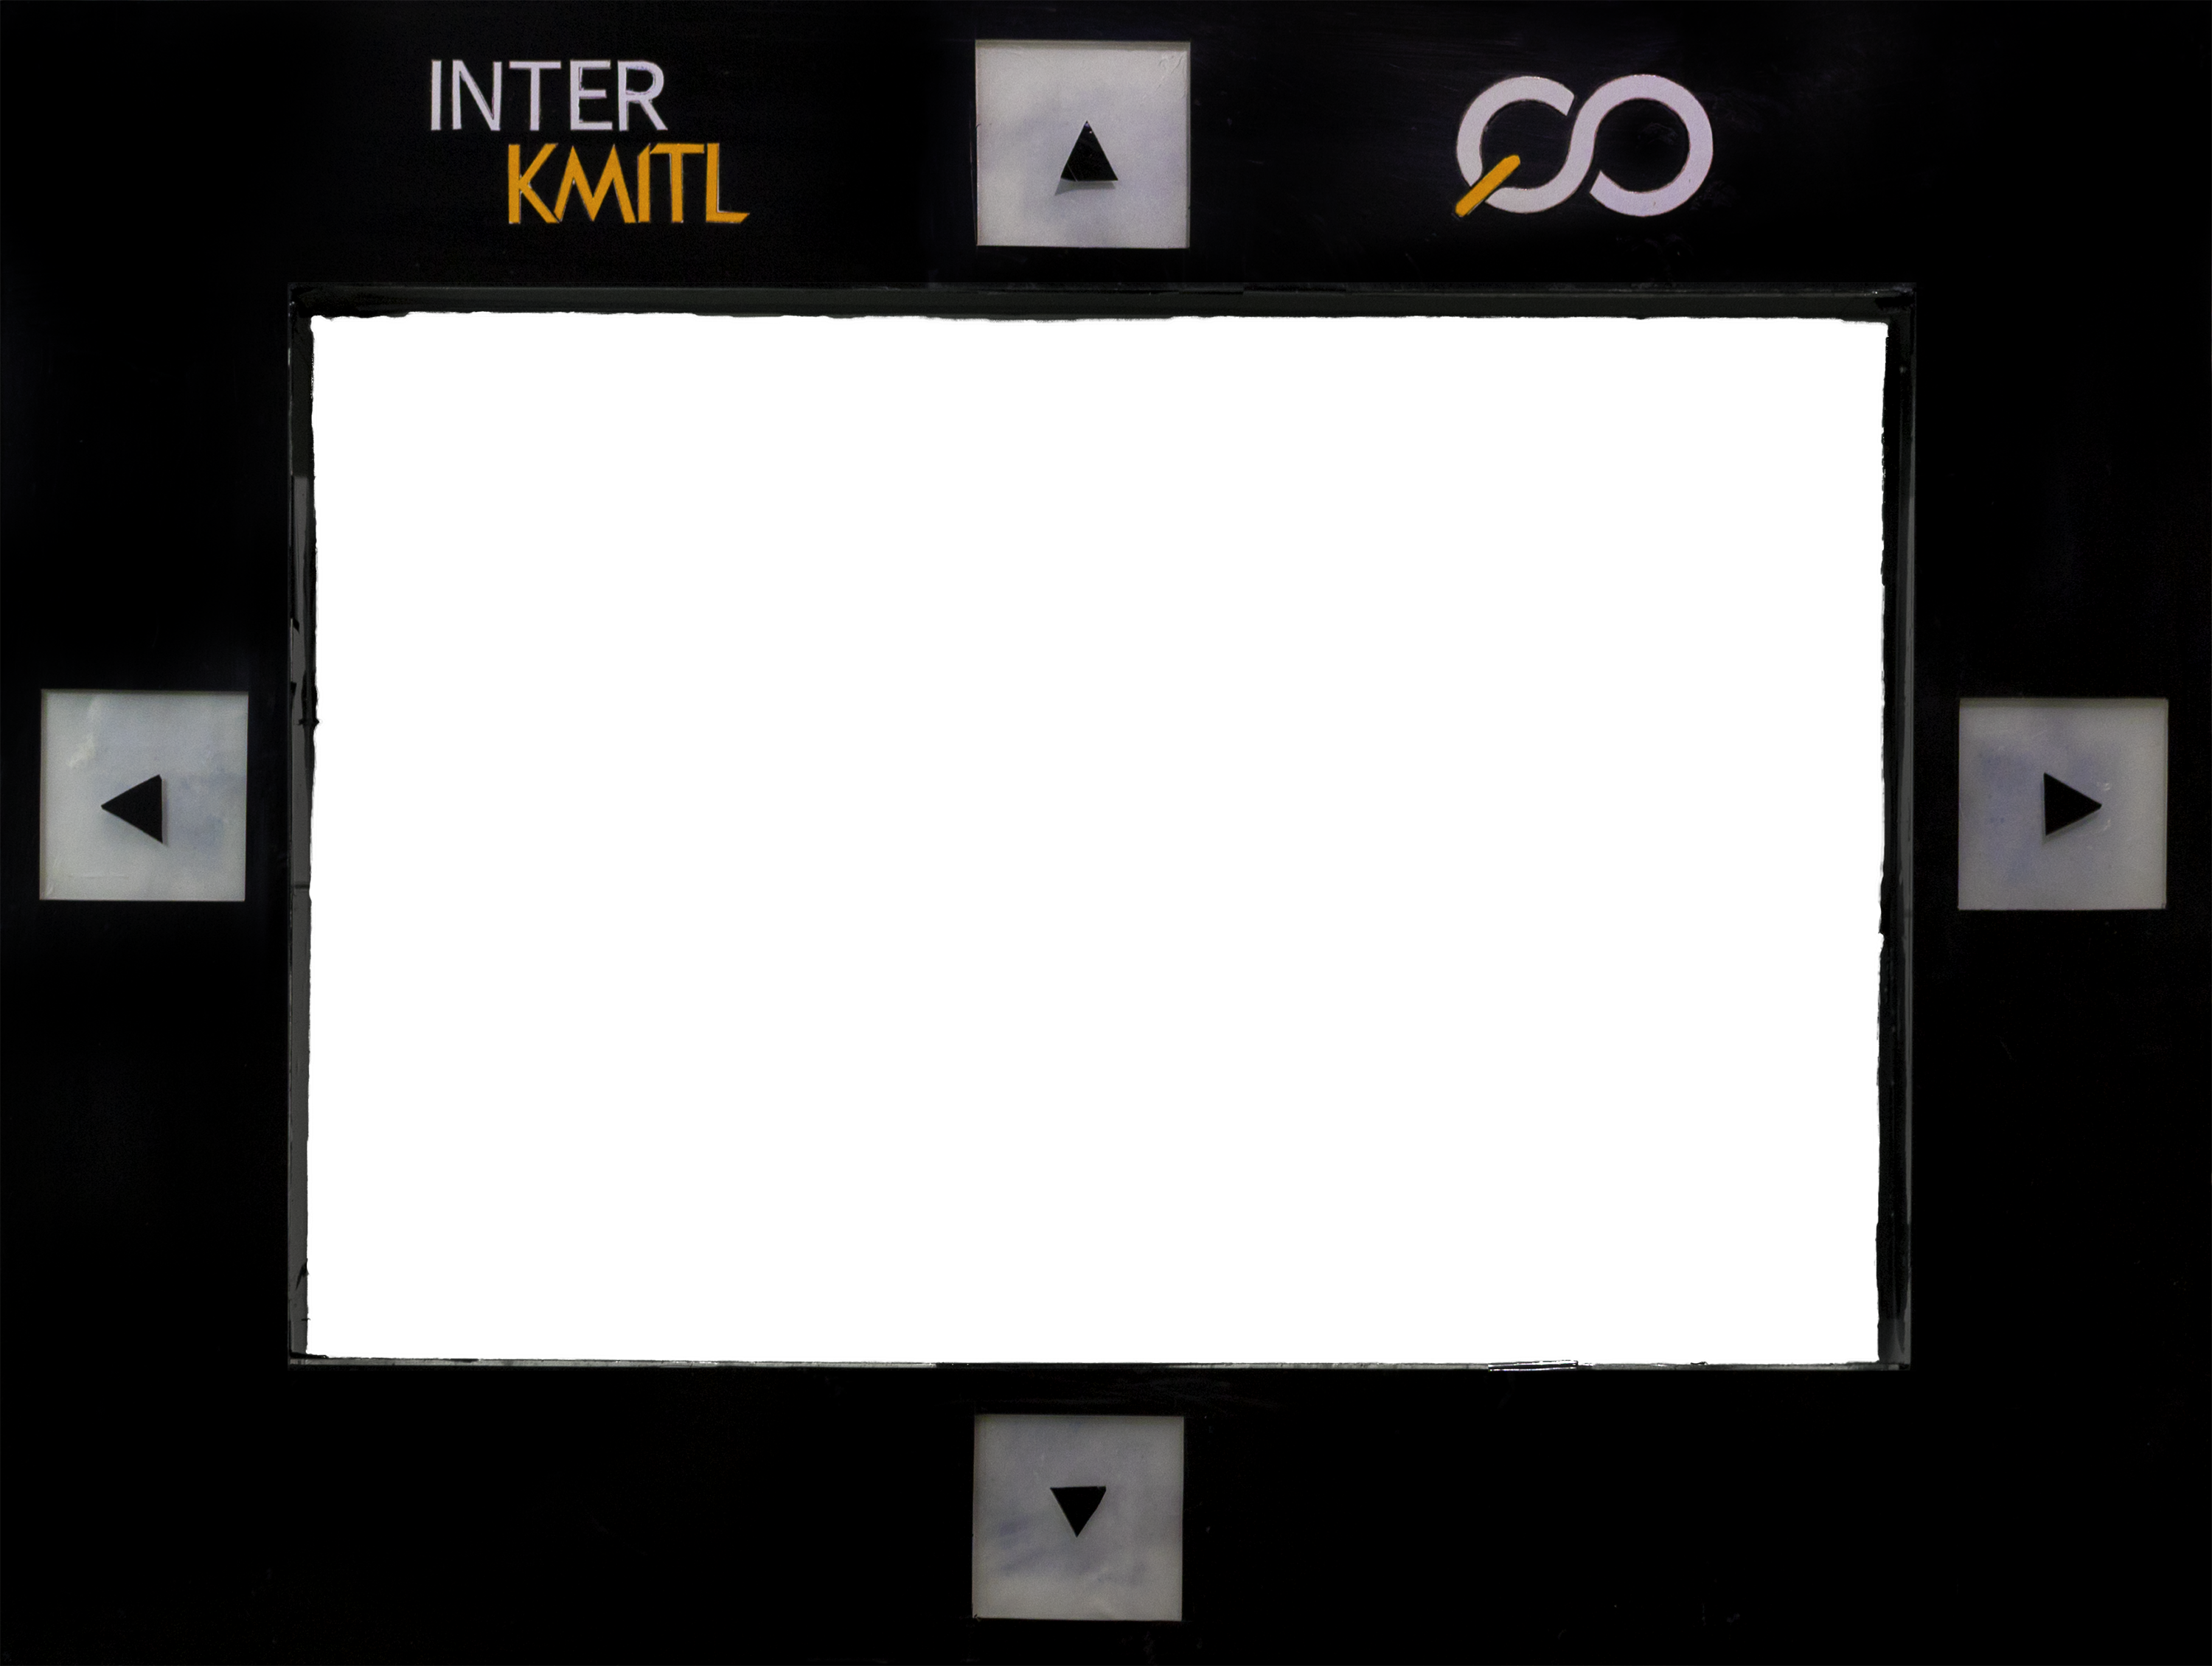
\includegraphics[width=\textwidth]{chapter7/frame.png}
	\caption{Visual Stimulator}
\end{figure}
\subsection{Visual stimulus (SSVEP)}

\section{Experiment I}

\subsection{Experiment Paradigm I}
\newcolumntype{P}[1]{>{\centering\arraybackslash}p{#1}}
\begin{table}[ht]
\centering
\begin{tabular}{| P{.3\linewidth} | P{.3\linewidth} | P{.3\linewidth} |}
			
			\hline 
			\textbf{Parameter} & \textbf{Experiment1}  & \textbf{Experiment2}\\
			\hline 
			Flickering type & Regular & Uniform random   \\
			\hline 
			Stimulus & Static & Modular  \\
			\hline 
			Sample Length & \multicolumn{2}{c}{64samples/epoch} \vline\\
			\hline 
			Epoch time & \multicolumn{2}{c}{500 ms} \vline\\
			\hline
		\end{tabular}
        
\caption{Experiment setting}
\label{table:2}
\end{table}

\subsection{Experiment II}

